\documentclass[11pt]{article}

\usepackage{amsmath,amssymb,amsthm}
\usepackage{graphicx,subcaption}
\usepackage{fullpage}
\usepackage{mathtools}
\usepackage{hyperref}
\usepackage{color}
\usepackage{blindtext}
\usepackage[dvipsnames]{xcolor}
\usepackage[shortlabels]{enumitem}
\usepackage{hyperref}     
\usepackage{url}         
\usepackage{xurl}         

\setlength\parindent{0pt}


\title{Convolutional Neural Network for DeepFake Detection}
\author{Abhinav Madabhushi, Pierce Ohlmeyer-Dawson}
\date{}

\begin{document}


\maketitle

\abstract{\blindtext}

\section{Introduction}
DeepFake classification is the process of identifying whether an image is real or AI-generated. According to some statistics, almost 0.1 percent of the images online are already fake, and if this goes on, the majority of the images on the internet will become fake. To moderate the fake images on the internet, it is important to have a model to classify whether a given image is fake or not, a task that is becoming more complicated by the day. Using technologies and generative models, it is extremely easy to produce an image similar to real life, and the human eye will not be able to tell the difference. As the models for generating AI images are growing, it is important to have content moderation, especially on social media websites, that recognizes and deletes these AI-generated images. Other applications of deepfake detection include news and media verification, law enforcement and digital forensics, identity verification, and cybersecurity and fraud detection, amongst many other applications. \\

There is also ongoing research that with repeated use of synthetic data (AI-generated images) in models, there is eventually going to be an irrecoverable model collapse, which would mean that models such as ChatGPT that have been trained for several years to reach their current state will have all its progress removed. This is due to the fact that every time synthetic data is generated, there are small perturbations to the image, and over time, the image degrades to an irrecoverable state. A lot of solutions have been proposed to mitigate this problem, out of which one solution is to create accurate deepfake detection models. Advanced convolutional neural network models are required for deepfake classification, especially for the fake images currently being made. 


\section{Background}
\subsection{Model Overview}

\noindent
\textbf{Input:} \( x \in \mathbb{R}^{H \times W \times C}\)  
(An RGB image with height \(H\), width \(W\), and \(C=3\))

\noindent
\textbf{Output:} \( y \in \mathbb{R}\)  
(0 or 1 output for binary classification)

\subsection{CNN Forward Propagation}

\paragraph{\normalsize Convolution Layer:}
For each output channel \(c'\) and spatial position \((x,y)\), compute
\[
z_{c'}(x,y) = h\!\Biggl( \sum_{c=1}^{C}\sum_{u=0}^{k-1} \sum_{v=0}^{k-1} x_c(x+u,y+v)\,w_{c',c}(u,v) + b_{c'} \Biggr),
\]
where \(h(\cdot)\) is a nonlinear activation function such as ReLU.

\paragraph{\normalsize Pooling Layer:}
Reduce the dimensions of the data by taking:
\[
p_{c'}(X,Y) = 
  \begin{cases}
    \displaystyle \max_{0 \le u,v < p}\, z_{c'}(pX+u,pY+v) & \text{(max pooling)} \\[2mm]
    \displaystyle \frac{1}{p^2}\sum_{0 \le u,v < p}\, z_{c'}(pX+u,pY+v) & \text{(average pooling)}
  \end{cases}
\]

\paragraph{\normalsize Fully Connected Layer:}
Flatten the pooled features into a vector \(p_d\) and compute:
\[
z_j^{(\mathrm{fc})} = h\!\Biggl( \sum_{d=1}^{D} w_{j d}^{(\mathrm{fc})} p_d + b_j^{(\mathrm{fc})} \Biggr).
\]

\paragraph{\normalsize Output Layer:}
\[
y = \sigma\!\Biggl( \sum_{j=1}^{M} w_{j}^{(\mathrm{out})} z_j^{(\mathrm{fc})} + b^{(\mathrm{out})} \Biggr),
\]
where \(\sigma\) is the sigmoid activation function for binary classification.

\subsection{CNN Backpropagation}

\paragraph{\normalsize Error Computation:}
At the output layer, the error is given by
\[
\delta_k^{(\mathrm{out})} = y_k - t_k,
\]
where \(t_k\) is the target.

\paragraph{\normalsize Gradient Computation:}

\paragraph{\normalsize Fully Connected Layer:}
\[
\delta_j^{(\mathrm{fc})} 
  = h'\!\Biggl( \sum_{d=1}^{D} w_{j d}^{(\mathrm{fc})} p_d + b_j^{(\mathrm{fc})} \Biggr)\,\sum_{k} w_{kj}^{(\mathrm{out})}\,\delta_k^{(\mathrm{out})},
\]
with the gradient of the weight computed as:
\[
\frac{\partial E}{\partial w_{jd}^{(\mathrm{fc})}} = \delta_j^{(\mathrm{fc})}\, p_{d}.
\]

\paragraph{\normalsize Pooling Layer:}
The gradient for the pooling layer is given by:
\[
\tilde{\delta}_{c'}(pX+u, pY+v) = 
\begin{cases}
\delta_{c'}^{(p)}(X,Y), & \text{if using max pooling and } z_{c'}(pX+u, pY+v) = p_{c'}(X,Y),\\[2mm]
0, & \text{if using max pooling and } z_{c'}(pX+u, pY+v) \neq p_{c'}(X,Y),\\[2mm]
\displaystyle \frac{1}{p^2}\,\delta_{c'}^{(p)}(X,Y), & \text{if using average pooling.}
\end{cases}
\]


\paragraph{\normalsize Convolutional Layer:}
Backpropagate the gradient as: 
\[
\delta_{c'}(x,y) = h'\!\Biggl( \sum_{c=1}^{C}\sum_{u=0}^{k-1} \sum_{v=0}^{k-1} x_c(x+u,y+v)\,w_{c',c}(u,v) + b_{c'} \Biggr)\,\tilde{\delta}_{c'}(x,y),
\]
and compute the gradient of the weight as:
\[
\frac{\partial E}{\partial w_{c',c}(u,v)} = \sum_{x,y} \delta_{c'}(x,y)\,x_c(x+u,y+v).
\]

\paragraph{\normalsize Weight update:}
Update weights using gradient descent
\[
w^{(\mathrm{new})} = w^{(\mathrm{old})} - \eta\, \frac{\partial E}{\partial w},
\]
where \(\eta\) is the learning rate. 

Similarly, back propagation is also performed on the bias term. 

\subsection{Conclusion}

Our CNN architecture integrates multiple convolutional and pooling layers for feature extraction and dimensionality reduction, followed by fully connected layers, and concludes with an output layer using a sigmoid activation for binary classification. \ref{ref:deeplearning}

\section{Dataset}

The dataset \ref{ref:kaggle} used in this project is a Kaggle dataset containing 60,000 real images from the CIFAR-10 dataset and 60,000 AI-generated synthetic images generated by Stable Diffusion version 1.4, a text-to-image generation model. The images are equivalent to those in the CIFAR-10 dataset, making them difficult to distinguish as Real or Synthetic. The real images from the CIFAR-10 dataset are widely used in academia and research, and the dataset is publicly released under specific terms that permit free use for non-commercial research. However, the fake images obtained from the stable diffusion model were trained on images scrapped from the internet, which could spark ethical issues of data privacy. Still, we are only using the output of that model for our model, which is not a major concern. There might be certain licensing and trademark issues with synthetic images replicating logos or distinctive product designs. There also might be bias in both the CIFAR-10 dataset and the stable diffusion data, as the dataset might contain only certain breeds of dogs and cats, for example, which might lead to the model not recognizing other breeds as fake or real. All these privacy, bias, and ethical concerns were taken into account before creating our CNN model. \\

Several preprocessing steps were taken for the dataset. Firstly, the data transformations and augmentations were done. Images in the training dataset had random horizontal flips with a 50 percent chance of getting flipped. Along with this, there were small random rotations of approximately 10 degrees and random alterations to brightness, contrast, saturation, and hue. This was done to give the training data diversity and to prevent overfitting. Secondly, data normalization and transformation were done. Each image in the dataset was made into a 32 by 32 image size with red, blue, and green (RGB) channels. The image's pixel values were normalized to a mean and standard deviation of 0.5. Then, the PIL images were converted to PyTorch tensors. Finally, the data was split into train, validation, and test datasets with an 80-10-10 split. \\

Basic exploratory data analysis was done on the data to observe what the real and fake images looked like. Five images were randomly chosen from the dataset and plotted using matplotlib.
\begin{figure}[htbp]
    \centering
    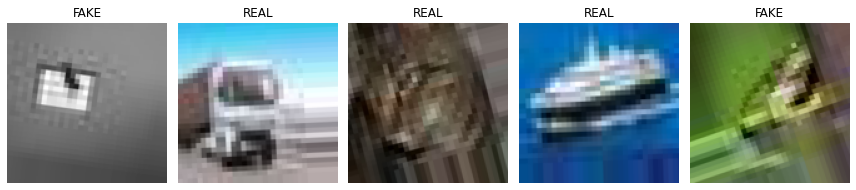
\includegraphics[width=0.8\textwidth]{EDA.png} 
    \caption{Visual inspections of images from the dataset}
    \label{fig:eda}
\end{figure}
As shown in Figure 1, the data is of extremely low quality, and this is because CIFAR-10 was derived from the “80 million tiny images” dataset, and researchers at that time chose 32×32 pixels in size because it significantly reduces storage and computational requirements, making it efficient to conduct research. \\Next, we analyzed the principal components of the features of the images. To do this, the images were run through a pre-trained model named VGG-16 to extract the features. We randomly sampled 160 images from the dataset for analysis and extracted its features. Then, the PCA was imported from the sklearn package in Python, and the principal components were analyzed. 
\begin{figure}[htbp]
    \centering
    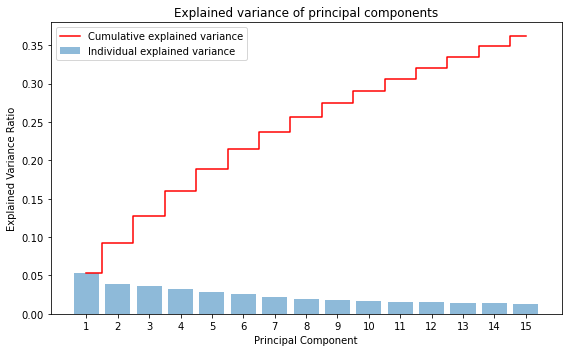
\includegraphics[width=0.4\textwidth]{PCA.png} 
    \caption{Principal Component Analysis}
    \label{fig:pca}
\end{figure}
As shown in Figure 2, even 15 components only explain approximately 35 percent of the variance in the dataset. Therefore, we decided to use all the features and instead used multiple pooling layers in our CNN architecture to reduce the number of dimensions. 

\section{Model}

\blindtext % Dummy text

\section{Methodology}

\blindtext % Dummy text

\section{Results}
\blindtext % Dummy text

\section{Conclusion}
\blindtext % Dummy text

\section{References}
\begin{enumerate}[label={[\arabic*]}]
    \item \label{ref:deeplearning} I. Goodfellow, Y. Bengio, and A. Courville, “Convolutional Networks,” in \textit{Deep Learning}. Cambridge, Massachusetts: MIT Press, 2016. [Online]. Available:  
    \url{https://www.deeplearningbook.org/contents/convnets.html}
    
    \item \label{ref:kaggle} J. J. Bird, “CIFAKE Real and AI-Generated Synthetic Images,” \textit{Kaggle}, 2023. [Online]. Available:  
    \url{https://www.kaggle.com/datasets/birdy654/cifake-real-and-ai-generated-synthetic-images}
\end{enumerate}

\end{document}